\documentclass[tikz,border=3pt]{standalone}
\usepackage[T1]{fontenc}
\usepackage{amsmath}\usepackage{graphicx}
\usepackage{XCharter}
\usepackage[xcharter]{newtxmath}
\usepackage[scaled=.92]{helvet}
\usepackage{pgfplots}
\usetikzlibrary{arrows.meta,positioning,fit,calc,backgrounds,decorations.pathreplacing,patterns}
\usepgfplotslibrary{groupplots,fillbetween}
\pgfplotsset{compat=1.18}
\definecolor{ink}{HTML}{172536}
\definecolor{rgb}{HTML}{3563B8}
\definecolor{event}{HTML}{17857C}
\definecolor{fusion}{HTML}{76529C}
\definecolor{reference}{HTML}{8994A3}
\definecolor{warn}{HTML}{AC5948}
\definecolor{muted}{HTML}{657183}
\definecolor{rule}{HTML}{D9E0E8}
\definecolor{pale}{HTML}{F5F7FA}
\color{ink}
\tikzset{box/.style={rounded corners=2pt,draw=rule,fill=white,align=center,inner sep=4pt,font=\sffamily\fontsize{9}{10.8}\selectfont,minimum height=9mm},rb/.style={box,draw=rgb!50,fill=rgb!5},eb/.style={box,draw=event!50,fill=event!5},fb/.style={box,draw=fusion!55,fill=fusion!5},arrow/.style={-{Latex[length=1.8mm]},line width=.65pt,draw=muted},note/.style={font=\sffamily\fontsize{8.4}{10.2}\selectfont,align=center,text=muted},heading/.style={font=\sffamily\fontsize{10}{12}\selectfont\bfseries,align=left,text=ink}}
\pgfplotsset{paper/.style={width=15.7cm,height=6cm,axis lines*=left,axis line style={rule},tick style={draw=none},tick label style={font=\sffamily\fontsize{8.8}{10.4}\selectfont,text=muted},label style={font=\sffamily\fontsize{9.4}{11}\selectfont,text=ink},title style={font=\sffamily\fontsize{10}{12}\selectfont\bfseries,text=ink},legend style={draw=none,fill=none,font=\sffamily\fontsize{9}{11}\selectfont,cells={anchor=west}},grid=major,grid style={rule!65,line width=.3pt},minor tick num=0,scaled ticks=false,unbounded coords=jump,clip mode=individual}}

\hyphenpenalty=10000\exhyphenpenalty=10000
\tikzset{box/.append style={font=\sffamily\fontsize{8}{10}\selectfont},
note/.append style={font=\sffamily\fontsize{8}{10}\selectfont}}
% Generated by scripts/make_official_results.py; do not edit by hand.
\providecommand{\OfficialPhasePublishedOverallMiD}{35.80}
\providecommand{\OfficialOverallAbsoluteGain}{9.228548419}
\providecommand{\OfficialBandContributionSubtotal}{9.227548419}
\providecommand{\OfficialDisplayRoundingResidual}{0.0010}
\providecommand{\OfficialCrucialSmallContributionShare}{82.4\%}
\providecommand{\OfficialPhaseOverallMiD}{35.8015}
\providecommand{\OfficialGarlOverallMiD}{45.03}
\providecommand{\OfficialOverallRelativeGain}{20.49\%}
\providecommand{\OfficialPhaseCrucialMiD}{43.5190}
\providecommand{\OfficialGarlCrucialMiD}{53.13}
\providecommand{\OfficialCrucialRelativeGain}{18.09\%}
\providecommand{\OfficialPhaseSmallMiD}{28.2568}
\providecommand{\OfficialGarlSmallMiD}{37.58}
\providecommand{\OfficialSmallRelativeGain}{24.81\%}
\providecommand{\OfficialPhaseLargeMiD}{25.7179}
\providecommand{\OfficialGarlLargeMiD}{40.61}
\providecommand{\OfficialLargeRelativeGain}{36.67\%}
\providecommand{\OfficialPhaseNegativeMiD}{29.9314}
\providecommand{\OfficialGarlNegativeMiD}{31.29}
\providecommand{\OfficialNegativeRelativeGain}{4.34\%}
\providecommand{\OfficialSampleCount}{6,762}
\providecommand{\OfficialPhaseFailureRate}{0.0\%}
\providecommand{\OfficialGarlFailureRate}{0.0\%}
\providecommand{\OfficialPhaseSubmissionID}{1016512}
\providecommand{\OfficialGarlSubmissionID}{817519}

\begin{document}

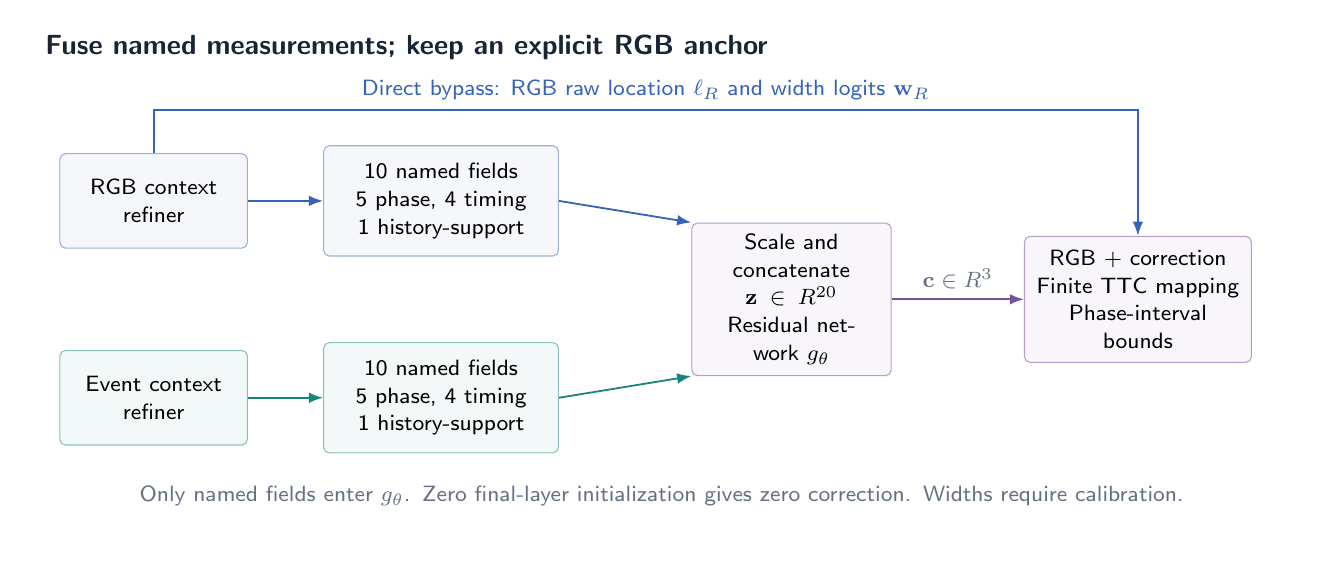
\begin{tikzpicture}[x=1cm,y=1cm]
\path[use as bounding box] (0,-.15) rectangle (16.2,6.3);
\node[heading,anchor=west] at (.1,6.05) {Fuse named measurements; keep an explicit RGB anchor};
\node[rb,text width=2.1cm,minimum height=12mm] (r) at (1.6,4.1) {RGB context\\refiner};
\node[eb,text width=2.1cm,minimum height=12mm] (e) at (1.6,1.6) {Event context\\refiner};
\node[rb,text width=2.7cm,minimum height=14mm] (rd) at (5.25,4.1) {10 named fields\\5 phase, 4 timing\\1 history-support};
\node[eb,text width=2.7cm,minimum height=14mm] (ed) at (5.25,1.6) {10 named fields\\5 phase, 4 timing\\1 history-support};
\node[fb,text width=2.25cm,minimum height=15mm] (g) at (9.7,2.85) {Scale and concatenate\\$\mathbf z\in\mathbb R^{20}$\\Residual network $g_\theta$};
\node[fb,text width=2.6cm,minimum height=16mm] (out) at (14.1,2.85) {RGB + correction\\Finite TTC mapping\\Phase-interval bounds};
\draw[arrow,rgb] (r)--(rd);
\draw[arrow,event] (e)--(ed);
\draw[arrow,rgb] (rd.east)--(g.north west);
\draw[arrow,event] (ed.east)--(g.south west);
\draw[arrow,fusion] (g.east)--node[above,note]{$\mathbf c\in\mathbb R^3$}(out.west);
\draw[arrow,rgb] (r.north)--(1.6,5.25)--node[above,note,text=rgb]{Direct bypass: RGB raw location $\ell_R$ and width logits $\mathbf w_R$}(14.1,5.25)--(out.north);
\node[note,text width=15.7cm] at (8.05,.35) {Only named fields enter $g_\theta$. Zero final-layer initialization gives zero correction. Widths require calibration.};
\end{tikzpicture}
\end{document}
